\section{Supporting Normalized Diagnostics}\label{app:normalized-diagnostics}

\subsection{Local response and a perturbation tool}
At a deterministic baseline $A_0=B(p)+\kappa I$ with degree matrix
$D_0$, perturb by $E=A-A_0$ and put
$C=D_0^{-1}\operatorname{diag}(E\mathbf1)$. Differentiation gives
\[
J_{A_0}(E)=D_0^{-1/2}ED_0^{-1/2}
-\tfrac12\{CS(p)+S(p)C\}.
\]
The two terms describe relation change and degree correction at the
same baseline. They are not an expansion around an arm-specific
expectation.

\begin{lemma}[Positive-degree perturbation bound]\label{lem:norm-perturbation}
Let $A,A'$ be symmetric nonnegative matrices, with row-sum diagonal
matrices $D,D'$ and minimum degree $d_0>0$ across both. Then
\[
\|D^{-1/2}AD^{-1/2}-D'^{-1/2}A'D'^{-1/2}\|_2
\le \frac{\|A-A'\|_2}{d_0}
+\frac{\|A'\|_2\|D-D'\|_2}{d_0^2}.
\]
\end{lemma}
\begin{proof}
Insert $D^{-1/2}A'D^{-1/2}$ and split the remaining normalization
difference into a left and a right factor. The scalar mean-value
bound $|x^{-1/2}-y^{-1/2}|\le|x-y|/(2d_0^{3/2})$ applies to
each diagonal entry. Each of the latter two terms is bounded by
$\|A'\|_2\|D-D'\|_2/(2d_0^2)$; the first is bounded by
$\|A-A'\|_2/d_0$.
\end{proof}
For a node-$u$ replacement, $|d_v-d'_v|$ is bounded by the number
of edge slots containing both $u$ and $v$. Including $v=u$ makes
the maximum of these counts equal to $\deg(u)$. The hub factor
must remain in the bound. Since $d_0\ge\kappa$, replacing $d_0$
by $\kappa$ is conservative, not an assertion of equality.

\subsection{Visual calibration protocol and conditional-risk analysis}\label{app:visual}
The visual objects use the ED-HNN preprocessing~\cite{wang2023edhnn} of NTU2012 and
ModelNet40. Input SHA-256 values are
\texttt{f59d6f62\ldots 30d2c} and \texttt{3de34493\ldots ee8b8} for
NTU2012 content and edges, and \texttt{51565c05\ldots 8604} and
\texttt{e6e0ae37\ldots 4048} for ModelNet40. The fixed stratified
split contains 1,182/377/453 NTU objects and 7,372/2,446/2,493
ModelNet objects (training/validation/test). The predictor uses hidden
width 64, Adam with learning rate 0.01 and weight decay
$5\times10^{-4}$, full-batch training and validation-loss
checkpointing. The epoch ceiling is 100 on NTU and 400 on ModelNet,
selected using ten development runs per dataset. Run seeds are
\texttt{2026102100 + dataset$\cdot10^5$ + batch$\cdot10^4$ +
role$\cdot10^3$ + index}; reference, calibration, evaluation and
development streams are disjoint. One batch per dataset contains
30/99/200 reference/calibration/evaluation complete runs. The
reference center is shared by all three calibrators and remains
frozen throughout their comparison.

Full counts, thresholds, tie rates, spectral residuals, timings and
input hashes are retained in the reproducibility materials under
\path{experiments/spectral-risk-calibration/results/visual_alarm_v1/}.
No spectral solver fallback occurred in the 658 complete training
runs. These caches preserve the distinction between independent
training runs and simulated draws from a fitted node or edge law.

\paragraph{Marginal and conditional probability targets.}
For a fixed reference center, let $\mathcal C$ denote the random
calibration sample and write
$r(\mathcal C)=\Pr_{\mathcal L}\{T_{\mathrm{new}}>q(\mathcal C)
\mid\text{reference},\mathcal C\}$.
Proposition~\ref{prop:rank} bounds the average over calibration
samples, $\mathbb E_{\mathcal C}r(\mathcal C)\le\alpha$.
A binomial tolerance rule instead bounds the calibration-sample
probability that $r(\mathcal C)$ exceeds $\alpha$.

The NTU frozen threshold gave 28/200 exceedances. With its reference
center fixed, 10,000 random 99/200 splits of the existing 299 scores
gave a mean of $5.0\%$, median $4.5\%$, and central $95\%$ range
$1.0$--$11.0\%$; $4.4\%$ of splits exceeded $10\%$. The frozen
threshold lay at the 0.4th percentile of resampled thresholds.
ModelNet gave mean $5.0\%$, median $4.5\%$, and central $95\%$ range
$1.0$--$11.0\%$. These averages describe repeated random partitions
of one finite score pool. Their agreement with the nominal target is
an internal rank-consistency check, not a new independent test of the
population guarantee. Uniform rounding of both score sets to 6--14
decimals changed the NTU count from 28 to 27 ($13.5\%$), so near ties
account for 0.5 percentage points of its observed rate.

\paragraph{Binomial tolerance calibration.}
For an independent-and-identically-distributed run mechanism,
conditional on the frozen reference stage, choose
\begin{equation}\label{eq:tolerance-order}
\begin{aligned}
k_{\alpha,\delta}
&=\min\bigl\{k\in\{1,\ldots,M\}:\\[-2pt]
&\hspace{1.5em}\Pr\{\operatorname{Binomial}(M,1-\alpha)\ge k\}
\le\delta\bigr\}.
\end{aligned}
\end{equation}
If no finite index satisfies the criterion, use an infinite threshold.
With $q=T_{(k_{\alpha,\delta})}$ and strict exceedance, the established
tolerance bound is
\[
\Pr_{\mathcal C}\{r(\mathcal C)>\alpha\mid\text{reference}\}
\le\delta
\]
\cite{vovk2012conditional}. This high-probability statement requires
the independent-run population model, rather than only the finite
exchangeability used for the marginal rank argument.

At $\alpha=\delta=.05$, the smallest admissible index is 98 for
$M=99$ (binomial tail 0.039), 195 for $M=199$ (0.027), 483 for
$M=499$ (0.035), and 961 for $M=999$ (0.044). At $M=99$, the marginal
rule instead takes index 95. Evaluating the tolerance threshold on
the same observed evaluation runs gives 19/200 ($9.5\%$) on NTU and
3/200 ($1.5\%$) on ModelNet. This comparison changes the probability
target and threshold, not the original frozen observations. Because
the comparison was chosen after observing the original evaluation
results, it does not supply an independent validation of the new
rule. Prospective use fixes $\alpha$, $\delta$, $M$ and the selection
criterion before new calibration and evaluation runs are generated.

\subsection{Secondary response to feature perturbations}\label{app:visual-response}
Each evaluation model was re-inferred on five paired feature-noise
strengths $\sigma\in\{0,.1,.25,.5,1\}$. Only non-training object
features were perturbed, with one Gaussian noise field shared across
strengths within each run; the candidate hypergraph, preprocessing,
model weights and reference center remained fixed. These experiments
compare score responses to this specified perturbation mechanism,
separately from the cross-domain calibration comparison in
Section~\ref{sec:visual}.

At $\sigma=1$ and a retrospective realized $10\%$ false-positive
rate, $T$ detection was $65.5\%$ on NTU versus $92.5\%$ for
Frobenius deviation (AUC 0.879 versus 0.976); on ModelNet it was
$66.5\%$ versus $100\%$ (AUC 0.925 versus 0.998), with predictive
entropy at $100\%$ (AUC 1.000). Observed $T$-minus-Frobenius
differences were $-27.0$ and $-33.5$ percentage points, with
paired-run percentile bootstrap $95\%$ intervals $[-36.5,-18.5]$ and
$[-41.0,-24.0]$, respectively. The curves use the same evaluation
scores for threshold selection and comparison, so they describe
in-sample ranking rather than calibrated deployment performance.

The two operator norms measure different functionals. For the
symmetric deviation $\Delta=S-\widehat M$,
\[
\|\Delta\|_2=\max_i|\lambda_i(\Delta)|,
\qquad
\|\Delta\|_F=\sqrt{\sum_i\lambda_i(\Delta)^2}.
\]
An increase spread across several spectral directions can therefore
raise Frobenius deviation more than the largest directional
component. This offers a possible explanation for the stronger
aggregate response under the tested Gaussian feature perturbations;
nonlinear prediction and normalization do not themselves imply an
isotropic operator perturbation. These measurements do not establish
an advantage for $T$ under localized or coherent changes, which would
require a separate comparison.

\begin{figure}[H]
\centering
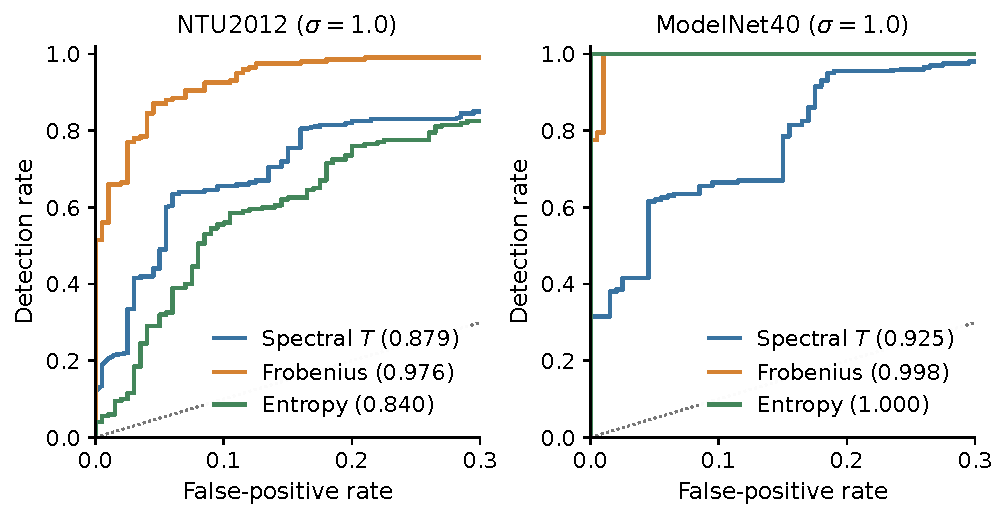
\includegraphics[width=\textwidth]{figures/visual_alarm_roc.pdf}
\caption{Secondary feature-perturbation comparison at $\sigma=1$.
Clean evaluation scores are negatives and paired perturbed scores are
positives. Thresholds are swept on the same evaluation data, so these
ROC curves describe score ranking rather than calibrated deployment
rules. The displayed interval is the low-false-positive-rate portion
of each curve; AUC values refer to the full curve.}
\label{fig:visual-alarm-roc}
\end{figure}
